\documentclass{sciposter}

\usepackage[utf8]{inputenc} % кодировка
\usepackage[english, russian]{babel} % Система переносов
\usepackage[T2A]{fontenc} % font encoding

\usepackage[pdftex]{graphicx} % images

% \usepackage{tempora} % шрифт Tempora (Tempora-TLF)
\usepackage{paratype} % шрифт PT Serif Caption (PTSerifCaption-TLF)

% mathematical formulas
\usepackage{amssymb}
\usepackage{amsmath}
\usepackage{amsfonts} % подкл. дополнительных мат. шрифтов
\usepackage{latexsym} % некоторые редкие символыs

\usepackage{multicol}

\title
{
    Равномерное распределение точек на сфере
}
\author
{
    И.Б.Рахимов \\
    Руководитель: О.Г.Корольков
}
\institute
{
    Воронежский Государственный Университет
}
\date
{
    \today
}
\email
{
    ihtier\_@outlook.com
}
\leftlogo
{
    images/vsu_logo.jpg
}
\rightlogo
{
    images/vsu_logo.jpg
}
\conference
{
    Студенческая конференция ЭФ ВГУ
}

\begin{document}

\maketitle

\begin{multicols}{3}

\begin{abstract}
Как можно более равномерное распределение точек на сфере — невероятно важная задача в математике, науке и компьютерных системах, а наложение сетки Фибоначчи на поверхность сферы при помощи равновеликой проекции — чрезвычайно быстрый и эффективный метод аппроксимации для её решения. В данной работе будет показано, как благодаря незначительным изменениям его можно сделать ещё лучше.
\end{abstract}

\section*{Введение}
\PARstart{З}{адача} равномерного распределения точек на сфере имеет очень долгую историю. Это одна из самых хорошо исследованных задач в математической литературе по сферической геометрии. Она имеет критическую важность во многих областях математики, физики, химии, в том числе в вычислительных методах, теории приближений, теории кодирования, кристаллографии, электростатике, компьютерной графике, морфологии вирусов и многих других.

К сожалению, за исключением нескольких особых случаев (а именно платоновых тел) невозможно идеально ровно распределить точки на сфере. Кроме того, решение задачи сильно зависит от критерия, который используется для оценки однородности. На практике используется множество критериев, в том числе:

\begin{itemize}
    \item Упаковка и покрытие;
    \item Выпуклые оболочки, ячейки Вороного и треугольники Делоне;
    \item Ядра $s$-энергии Риса;
    \item Кубатура и определители.
\end{itemize}

Очень важно уяснить этот аспект: обычно не существует единственного оптимального решения этой задачи, потому что оптимальное решение, основанное на одном критерии, часто не является оптимальным распределением точек для других. Например, мы также выясним, что оптимизация упаковки необязательно создаёт оптимальную выпуклую оболочку и наоборот.

\section{Оптимизация расстояния упаковки}

Часто эту задачу называют задачей Тэммса в честь ботаника Тэммса, искавшего объяснение структуры поверхности пыльцевых зёрен. Критерий упаковки требует от нас максимизировать наименьшее расстояние между соседями для $N$ точек. То есть:

\begin{displaymath}
    d_N = \min_{i \neq j} \Vert x_i - x_j \Vert _2,
\end{displaymath}

\noindent это значение уменьшается со скоростью $\dfrac{1}{\sqrt{N}}$, поэтому полезно будет определить нормализованное расстояние, а также асимптотический предел нормализованного расстояния как:

\begin{displaymath}
    d^*_N = \sqrt{N} d_N,
    \qquad
    d^* = \lim_{N \rightarrow \infty} d^*_N.
\end{displaymath}

\section{Сетка Фибоначчи}

Одно очень элегантное решение моделирует узлы, встречающиеся в природе, это явление называется спиральным филлотаксисом. Коксетер показал, что такие структуры имеют фундаментальную связь с рядом Фибоначчи:

\begin{displaymath}
    F_k = \{1, 1, 2, 3, 5, 8, 13, \ldots \}
\end{displaymath}

\noindent и золотым сечением:

\begin{displaymath}
    \phi = \frac{1 + \sqrt{5}}{2}.
\end{displaymath}

В литературе встречается два схожих определения множества точек сферической сетки Фибоначчи. Исходное определено строго для $N$, равного одному из членов ряда Фибоначчи, $F_m$, и хорошо изучено в теории чисел:

\begin{displaymath}
    t_i = \left( \frac{i}{F_m}, \frac{i \cdot F_{m-1}}{F_m} \right),
    \qquad
    0 \leq i \leq N-1.
\end{displaymath}

Второе определение, при котором $d^* = 2$, обобщает формулу до произвольного количества $N$ и используется в вычислениях чаще:

\begin{displaymath}
    t_i = \left( \frac{i}{N}, \frac{i}{\phi} \right),
    \qquad
    0 \leq i \leq N-1,
    \tag{1}
\end{displaymath}

\begin{displaymath}
    \phi = \frac{1 + \sqrt{5}}{2} = \lim_{n \rightarrow \infty} \left( \frac{F_{n+1}}{F_n} \right).
\end{displaymath}

% h    Place the float here, i.e., approximately at the same point it occurs in the source text (however, not exactly at the spot)
% t    Position at the top of the page.
% b    Position at the bottom of the page.
% p    Put on a special page for floats only.
% !    Override internal parameters LaTeX uses for determining "good" float positions.
% H    Places the float at precisely the location in the LaTeX code. Requires the float package (\usepackage{float}). This is somewhat equivalent to h!.
\begin{figure}[H]
    \centering
    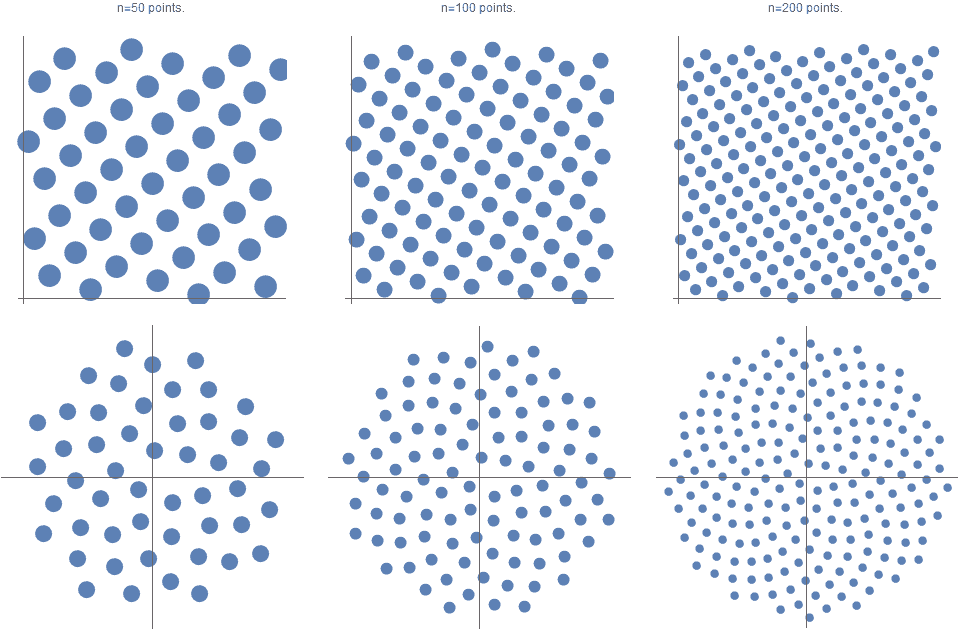
\includegraphics[width=\textwidth]{images/1.png}
    \caption{Примеры сеток Фибоначчи}
\end{figure}


\section*{Сетка 1}
\addcontentsline{toc}{subsubsection}{Сетка 1} % toc - table of contents

Более распространённая версия (особенно в компьютерных системах), создающая более хорошее значение $d^*=3.09$, имеет вид:

\begin{displaymath}
    t_i = \left( \frac{i + 0.5}{N}, \frac{i}{\phi} \right),
    \qquad
    0 \leq i \leq N-1.
    \tag{2}
\end{displaymath}

Она располагает точки в средних точках интервалах (по правилу средней точки в квадратной формуле Гаусса), поэтому для $n=100$, значения первой координаты будут такими:

\begin{displaymath}
    \{
        \frac{0.5}{100},
        \frac{1.5}{100},
        \frac{2.5}{100},
        \ldots,
        \frac{97.5}{100},
        \frac{98.5}{100},
        \frac{99.5}{100}
    \}.
\end{displaymath}

\section*{Сетка 2}
\addcontentsline{toc}{subsubsection}{Сетка 2} % toc - table of contents

Ключевым моментом для дальнейшего улучшения уравнения 2, является осознание того, что $d^*_N$ всегда соответствует расстоянию между точками $t_0$ и $t_3$, которые находятся на полюсах. То есть для улучшения $d_N$ точки рядом с полюсами должны быть разнесены ещё дальше.

Если мы определим следующее распределение:

\begin{displaymath}
    t_i = \left( \frac{i + \varepsilon}{N - 1 + 2 \varepsilon}, \frac{i}{\phi} \right),
    \qquad
    0 \leq i \leq N-1,
\end{displaymath}

\noindent $d^*_N$ — кривые для различных значений. $\varepsilon=0$ (синяя); $\varepsilon=\dfrac{1}{2}$ (оранжевая); $\varepsilon=\dfrac{3}{2}$ (зелёная); и $\varepsilon=\dfrac{5}{2}$ (красная). Можно увидеть, что $\varepsilon = \dfrac{5}{2}$ даёт результаты ближе к асимптотическим результатам. То есть при $N>20$ следующее простое выражение генерирует значительно более хорошие результаты $d^* = 3.29$ по сравнению с канонической сферической сеткой Фибоначчи:

\begin{displaymath}
    t_i = \left( \frac{i + 1.5}{N + 3}, \frac{i}{\phi} \right),
    \qquad
    0 \leq i \leq N-1.
    \tag{3}
\end{displaymath}

То есть при $N=100$ значения первой координаты будут равны:

\begin{displaymath}
    \{
        \frac{1.5}{103},
        \frac{2.5}{103},
        \frac{3.5}{103},
        \ldots,
        \frac{98.5}{103},
        \frac{99.5}{103},
        \frac{100.5}{103}
    \}.
\end{displaymath}

\begin{figure}[H]
    \centering
    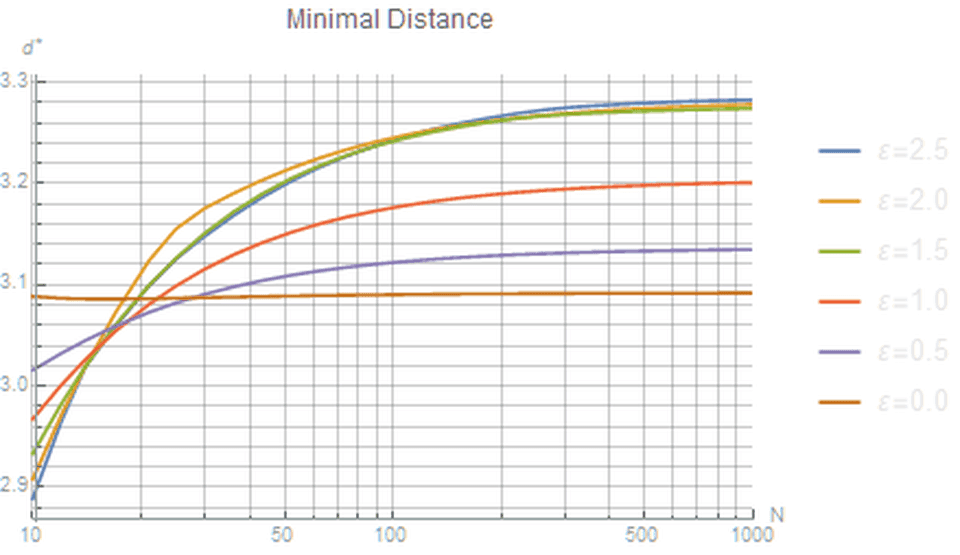
\includegraphics[width=\textwidth]{images/2.png}
    \caption{Различные значения $d_N^*$ при разных значениях $\epsilon$. Чем больше значение, тем оптимальнее конфигурации. Мы видим, что $\epsilon \simeq 2.5$ обеспечивает решение, близкое к оптимальному.}
\end{figure}

\section*{Сетка 3}
\addcontentsline{toc}{subsubsection}{Сетка 3} % toc - table of contents

Как сказано выше, одна из самых серьёзных проблем равномерного распределения точек на сфере заключается в том, что оптимальность распределения критически зависит от используемой целевой функции. Оказывается. что локальные величины наподобие $d_N^*$ иногда почти «не прощают ошибок» — единственная точка в недостаточно оптимальной позиции может катастрофически снизить оценку всего распределения точек.

В нашем случае вне зависимости от величины $N$ значение $D_N^*$ обычно определяется четырьмя точками, наиболее близкими к каждому из полюсов, особенно $t_0$ и $t_3$. Однако об этой сетке также известно то, что наибольший многоугольник Вороного находится на полюсе. Таким образом, пытаясь максимизировать $d_N$ разделением изначальных полярных точек в ряду, мы на самом деле ещё больше увеличиваем пустоту на полюсе! Поэтому мы представили альтернативу сетке 2, которая в общем случае более предпочтительна, потому что она не демонстрирует такой большой пустоты рядом с полюсами.

Она почти идентична сетке 2, но имеет два отличия. Во-первых, она использует $\varepsilon = \dfrac{11}{2}$ при $1 \leq i \leq N-2$. Во-вторых, кроме этих $N-2$ точек первая и последняя точки располагаются на каждом из полюсов.

То есть:

\begin{displaymath}
    t_0 = (0, 0),
    \qquad
    t_{N-1} = (1, 0),
\end{displaymath}

\begin{displaymath}
    t_i = \left( \frac{i + 3.5}{N + 6}, \frac{i}{\phi} \right),
    \qquad
    0 \leq i \leq N-1.
    \tag{4}
\end{displaymath}

\begin{figure}[H]
    \centering
    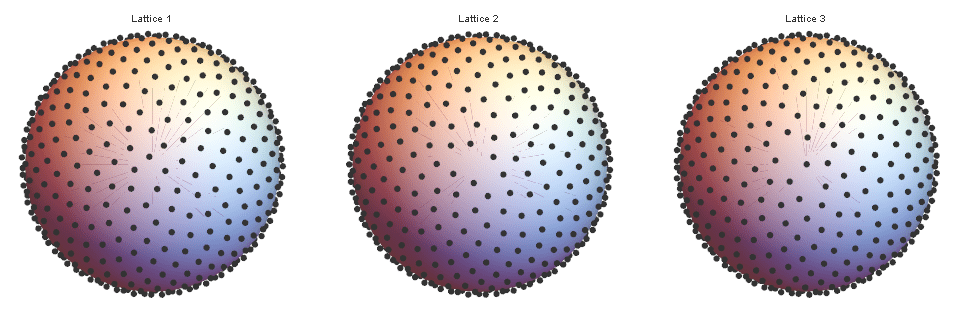
\includegraphics[width=\textwidth]{images/3.png}
    \caption{Различные конфигурации сеток. Каноническая сетка Фибоначчи слева. Заметьте, что несмотря на то, что у средней сетки $d_N^*$ улучшено, на полюсе у неё есть заметная пустота. Сетка 3 не имеет пустоты на полюсе и обладает наилучшим значением $d_N^*$.}
\end{figure}

\section{Вывод}

Сетка, соответствующая уравнению 6, является модификацией канонической сетки Фибоначчи, создающей значительно лучшее распределение точек, исходя из объёма и площади поверхности выпуклой оболочки (сетки Делоне).

\bibliographystyle{gost705}  % gost705-2008
\nocite{*}  % включение в список литературы всех записей из базы данных
\bibliography{sources}         % bib-files

\end{multicols}

\end{document}